\documentclass[a4paper, 12pt]{article}
\usepackage[a4paper,top=1.5cm, bottom=1.5cm, left=1cm, right=1cm]{geometry}
\usepackage{cmap}					% поиск в PDF
\usepackage{mathtext} 				% русские буквы в формулах
\usepackage[T2A]{fontenc}			% кодировка
\usepackage[utf8]{inputenc}			% кодировка исходного текста
\usepackage[english,russian]{babel}	% локализация и переносы

\usepackage{amsmath}
\usepackage{indentfirst}
\usepackage{longtable}
\usepackage{graphicx}
\usepackage{array}

\usepackage{wrapfig}
\usepackage{siunitx} % Required for alignment
\usepackage{subfigure}
\usepackage{multirow}
\usepackage{rotating}
\usepackage{caption}
\usepackage{subcaption}

\graphicspath{{img/}}
\usepackage{fancyhdr}
\usepackage{lastpage}
\pagestyle{fancy}
\fancyhf{}
\fancyhead[L]{ФРКТ}
\fancyhead[R]{Петля Гистерезиса}
\fancyfoot[C]{Артем Шилов}

\title{\begin{center}Лабораторная работа №3.4.5\end{center}
Петля гистерезиса (Динамический метод)}
\author{Шилов Артем Витальевич\\}
\date{Сентябрь 2024}

\begin{document}
    \pagenumbering{gobble}
    \maketitle
    

\section{Обработка результатов}
Данные нашей установки: \\
$R_0 = 0,3 \text{ Ом}, R_u = 20 \text{ кОм}, C_u = 20 \text{ мкФ}$

\subsection{Феррит 1000 нм} \\
\\ Изначально заданные нам условия: 
    $N_0 = 40 \text{ Витков},$ $ N_U = 400 \text{ Витков}, $ $ S = 3,0 \text{ см}^2, $ $ 2 \pi R = 25 \text{ см}$ \\
Данные полученные в ходе измерений:
\begin{center}
\begin{tabular}{|r|l|l|}
\hline
\multicolumn{1}{|l|}{I, mA} & x, дел & y, дел \\ \hline
100                         & 5,2    & 3,5    \\ \hline
90                          & 5      & 3,2    \\ \hline
80                          & 4,5    & 3      \\ \hline
72                          & 4      & 2,6    \\ \hline
61,3                        & 3,5    & 2,5    \\ \hline
52,1                        & 2,9    & 2,2    \\ \hline
40,9                        & 2,3    & 1,8    \\ \hline
31,4                        & 1,8    & 1,2    \\ \hline
21                          & 1,5    & 0,8    \\ \hline
16                          & 1,1    & 0,5    \\ \hline
\end{tabular}
\end{center}
Изображение петли гистерезиса для феррита на ЭО: 
\begin{center}
    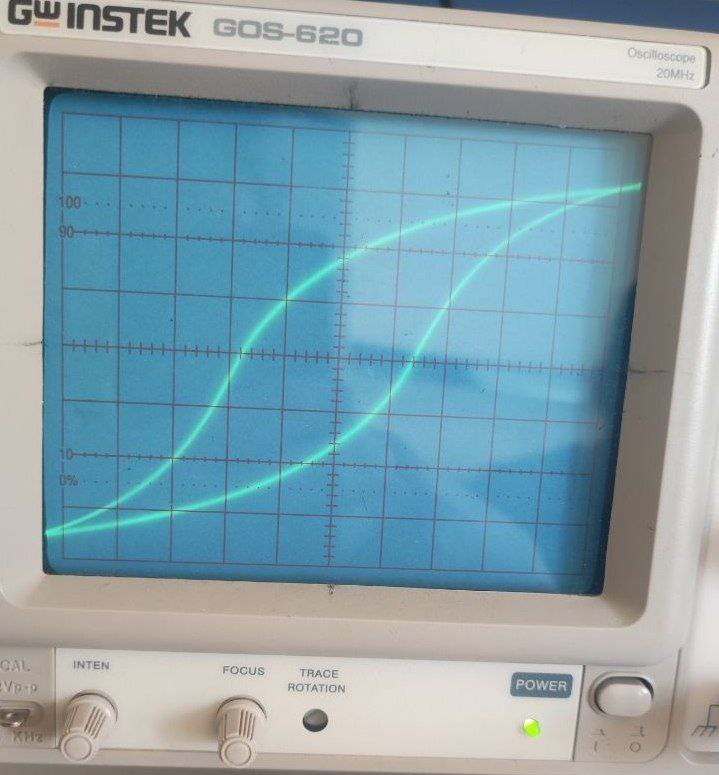
\includegraphics[width=0.4\linewidth]{Ferrit.jpg}
    \caption{Рис. 1}
    \label{fig:enter-label}
\end{center}
Посчитаем искомые значения:
$$H = \frac{I N_0}{2 \pi R} = 16 \text{ А/м}, H_c = 4.5 \text { А/м}$$
$$B = \frac{R_u C_u U_\text{вых}}{S N_U} = 0.19 \text{ Тл}, B_s = 1.1 \text{ Тл}$$
$$I_\text{эф} = 0.1 \text{ А}, K_x = 1, K_y = 20$$
$$2x(c) = 10.4 \text{ дел}, \phantom 22y(c) = 7 \text{ дел}$$
Построим на основе наших измерений график: 
\begin{center}
    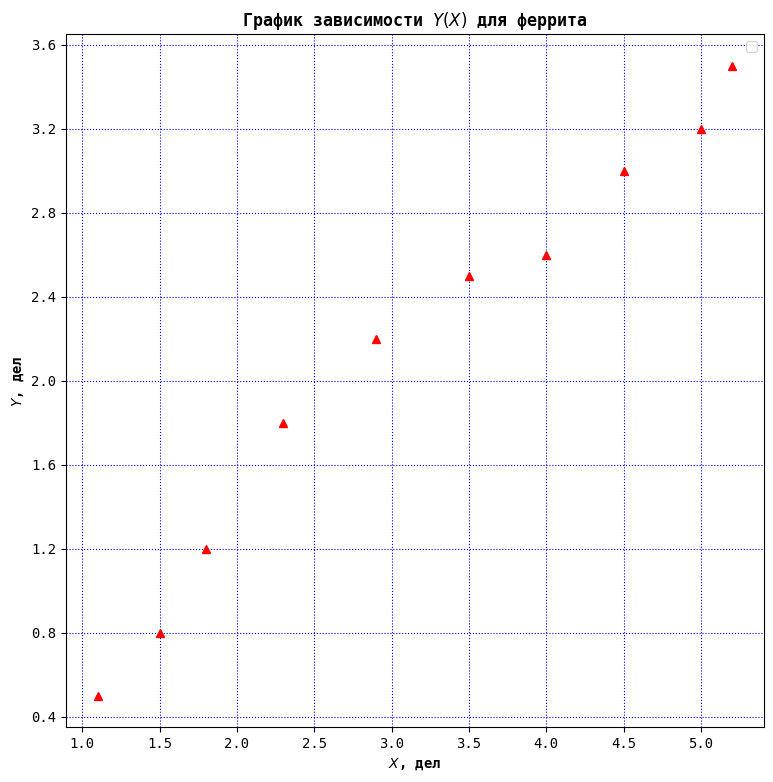
\includegraphics[width=0.5\linewidth]{Ferrit_graphic.png}
    \caption{Рис. 2}
    \label{fig:enter-label}
\end{center}

\subsection{Пермаллой}
\\ Изначально заданные нам условия: 
    $N_0 = 35 \text{ Витков},$ $ N_U = 220 \text{ Витков}, $ $ S = 3,8 \text{ см}^2, $ $ 2 \pi R = 24 \text{ см}$ \\
Данные полученные в ходе измерений:
\begin{center}
\begin{tabular}{|r|r|r|}
\hline
\multicolumn{1}{|l|}{I, mA} & \multicolumn{1}{l|}{x, дел} & \multicolumn{1}{l|}{y, дел} \\ \hline
96,3                        & 4                           & 4,3                         \\ \hline
89,9                        & 3,8                         & 3,4                         \\ \hline
83,2                        & 3,5                         & 2,5                         \\ \hline
76                          & 3,3                         & 2                           \\ \hline
71                          & 3,1                         & 1,5                         \\ \hline
64                          & 3                           & 1                           \\ \hline
50                          & 2,8                         & 0,7                         \\ \hline
41,7                        & 2,3                         & 0,5                         \\ \hline
35                          & 2                           & 0,3                         \\ \hline
24,5                        & 1,5                         & 0,2                         \\ \hline
\end{tabular}
\end{center}
Изображение петли гистерезиса для пермаллойа на ЭО:
\begin{center}
    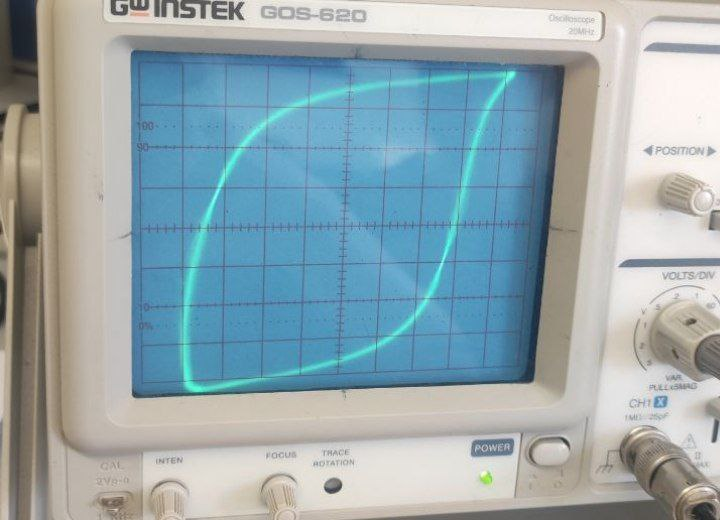
\includegraphics[width=0.5\linewidth]{Permalloy.jpg}
    \caption{}
    \label{fig:enter-label}
\end{center}
Посчитаем искомые значения:
$$H = \frac{I N_0}{2 \pi R} = 14 \text{ А/м}, H_c = 0.23\text{ А/м}$$
$$B = \frac{R_u C_u U_\text{вых}}{S N_U} = 0.27 \text{ Тл}, B_s = 1.4\text{ Тл}$$
$$I_\text{эф} = 0.0963 \text{ А}, K_x = 1, K_y = 20$$
$$2x(c) = 8 \text{ дел}, \phantom 22y(c) = 8.6 \text{ дел}$$Построим на основе наших измерений график: 
\begin{center}
    \centering
    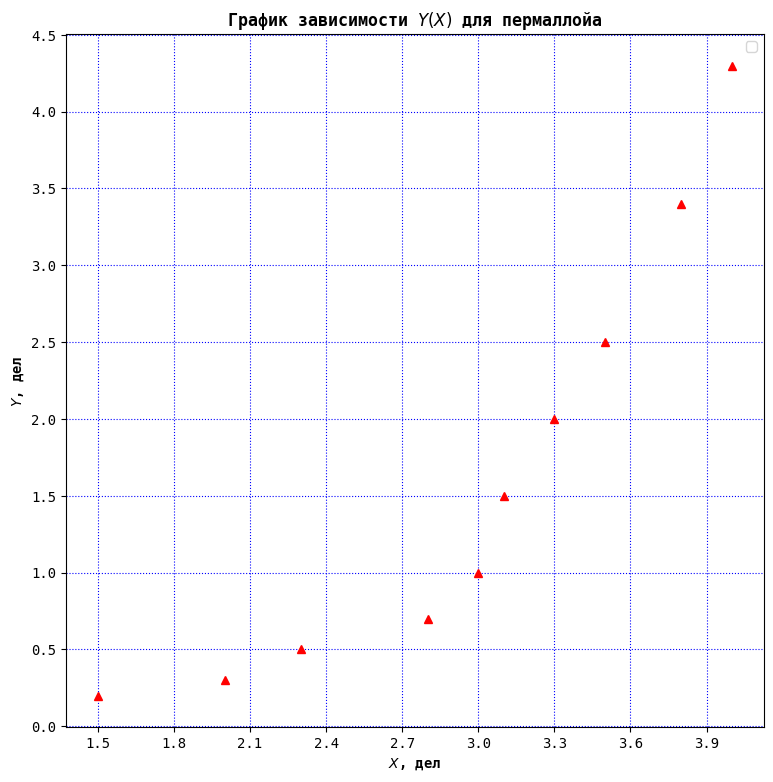
\includegraphics[width=0.5\linewidth]{Permalloy_graphic.png}
    \caption{Рис. 3}
    \label{fig:enter-label}
\end{center}

\subsection{Кремнистое железо}
\\ Изначально заданные нам условия: 
    $N_0 = 40 \text{ Витков},$ $ N_U = 400 \text{ Витков}, $ $ S = 1,2 \text{ см}^2, $ $ 2 \pi R = 10 \text{ см}$ \\
Данные полученные в ходе измерений:
\begin{center}
\begin{tabular}{|r|r|r|}
\hline
\multicolumn{1}{|l|}{I, mA} & \multicolumn{1}{l|}{x, дел} & \multicolumn{1}{l|}{y, дел} \\ \hline
75                          & 3,6                         & 4                           \\ \hline
68                          & 3,2                         & 3,5                         \\ \hline
60                          & 3                           & 3                           \\ \hline
52,7                        & 2,3                         & 2,3                         \\ \hline
45                          & 2                           & 1,8                         \\ \hline
38,6                        & 1,7                         & 1,3                         \\ \hline
31,8                        & 1,4                         & 1                           \\ \hline
26                          & 1                           & 0,7                         \\ \hline
21,3                        & 0,8                         & 0,5                         \\ \hline
16                          & 0,6                         & 0,3                         \\ \hline
\end{tabular}
\end{center}
Изображение петли гистерезиса для кремнистого железа на ЭО:
\begin{center}
    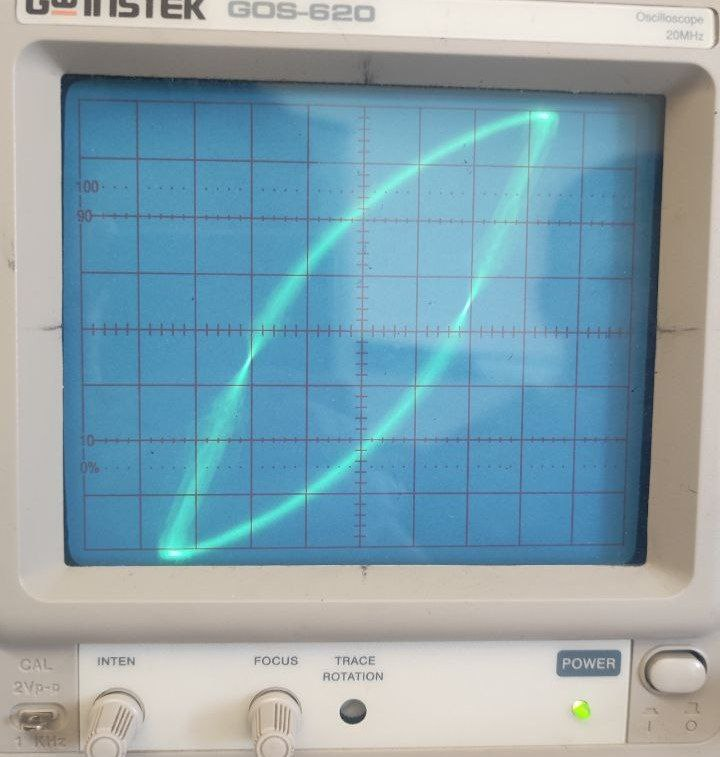
\includegraphics[width=0.5\linewidth]{Cremnistoe_iron.jpg}
    \caption{}
    \label{fig:enter-label}
\end{center}
Посчитаем искомые значения:
$$H = \frac{I N_0}{2 \pi R} = 30 \text{ А/м}, H_c = 4.5\text{ А/м}$$
$$B = \frac{R_u C_u U_\text{вых}}{S N_U} = 0.475 \text{ Тл}, B_s = 1.1 \text{Тл}$$
$$I_\text{эф} = 0.075 \text{ А}, K_x = 1, K_y = 20$$
$$2x(c) = 7.2 \text{ дел}, \phantom 22y(c) = 8 \text{ дел}$$
Построим на основе наших измерений график: 
\begin{center}
    \centering
    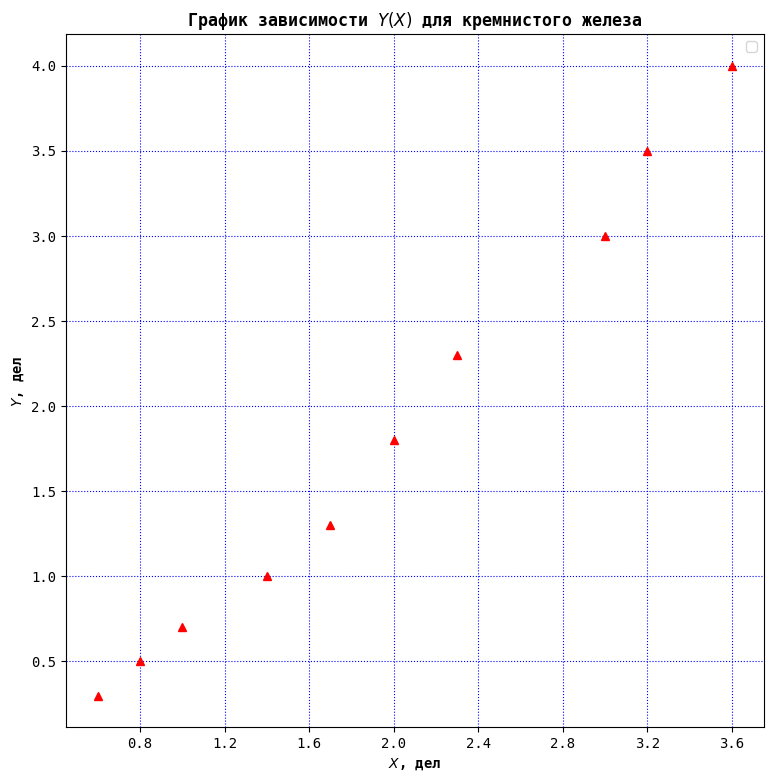
\includegraphics[width=0.5\linewidth]{iron_graphic.png}
    \caption{Рис. 4}
    \label{fig:enter-label}
\end{center}
\subsection{Расчет постоянной времени цепи}
$$\tau = RC = \frac{U_\text{вх}}{\Omega * U_\text{вых}} = 0.32 \pm 0.09 \text{ с}$$
Расчитывай параметры цепи $\tau = R_u * C_u = 0.4$ с, что близко к полученному резульату.
\section{Вывод}
В рамках данной лабораторной работы были изучены петли гистерезиса для трех разных образцов, и для каждого из них были получены характерные величины, которые по порядку величины совпали с табличными значениями. Также была оценена применимость используемого метода в условиях нашего эксперимента. В результате было подтверждено, что условия применимости соблюдаются, а сам метод является эффективным для определения характерных параметров ферромагнитных материалов.
\end{document}
